% ==============================================================================
% TCC - Gabriel dos Santos Sereno
% Capítulo 3 - Metodologia da construção do modelo
% ==============================================================================
\chapter{Metodologia da construção do modelo}
\label{sec-requisitos}

A metodologia apresentada aplica informações provenientes de máquinas de processamento químico, com objetivo de identificar quaisquer falhas no decorrer do processo.

Inicialmente, os dados são coletados da maquina, como o volume dos produtos químicos utilizados, temperatura, abertura de válvula e varias outras características. Com o controle de cada característica e modificando-as intencionalmente, é possível gerar falhas e assim, agrupar os dados gerados e rotula-los de acordo com a falha apresentada. Então, para cada falha rotulada nesse conjunto de dados, um classificador é especializado em identificar a falha selecionada. Esse conjunto de dados é introduzido em todos os classificadores, embora, a classe positiva é correspondente falha, permanecendo as demais classes como negativa.

Com o objetivo de diagnosticar as falhas, a metodologia proposta foca em características que mais se manifesta durante a ocorrência da falha e o identifica de acordo com o padrão dos dados. Portanto, foi utilizado selecionadores de características para realizar um comparativo, a respeito de qual deles detectam melhor essa variação quando está ocorrendo a falha.

A aplicação dessa proposta está descrito no Capítulo \ref{sec-projeto}, onde foram aplicados em duas máquinas de processo químico para comparar tais selecionadores de características. Nas próximas subseções, é descrito como foi preparado os dados, selecionadores, classificadores e também todos outros detalhes relevantes para a construção completa do modelo.

\section{Dados para os classificadores}

Os dados para os classificadores proposto nessa metodologia é separado em duas bases entre treinamento e testes. Entretanto, não foram divididos igualmente, pois a base de treinamento requer mais dados para possibilite que os classificadores aprenderem o padrão dos dados e assim classifica-los. Portanto, os dados de teste servem para metrificar a eficiência de um determinado classificador com dados novos e nunca introduzidos no classificador.

\section{Decomposição dos dados multi-classe}

Após a divisão dos dados em bases de treinamento e de testes, ambos precisão ser decompostos, de acordo com a metodologia proposta. Para isso, deve-se modificar a rotulação dos dados multi-classe para binário. Para isso, cada caso analisado neste presente estudo cientifico, foi criado, de acordo com o número de classes, bases iguais, mas com rótulos diferentes. Para melhor entendimento, caso o estudo fosse baseado nos dados das flores Iris, onde temos três tipos de flores, seriam feitos três novas bases para essas três classes, entretanto, a rotulação é diferente para cada base, como ilustra a figura \ref{fig-flores}. Com isso, para a primeira flor, os dados que correspondem a segunda e a terceira flor, seriam rotulados como dados negativos e para a primeira, positivos e assim por diante. Portanto, em cada estudo foram divididos em sub-bases binárias, tanto a base de treinamento, tanto a de teste para que cada classificador seja especializado em identificar apenas um tipo de falha.

\usetikzlibrary{positioning}

\begin{figure}[ht]
    \centering
    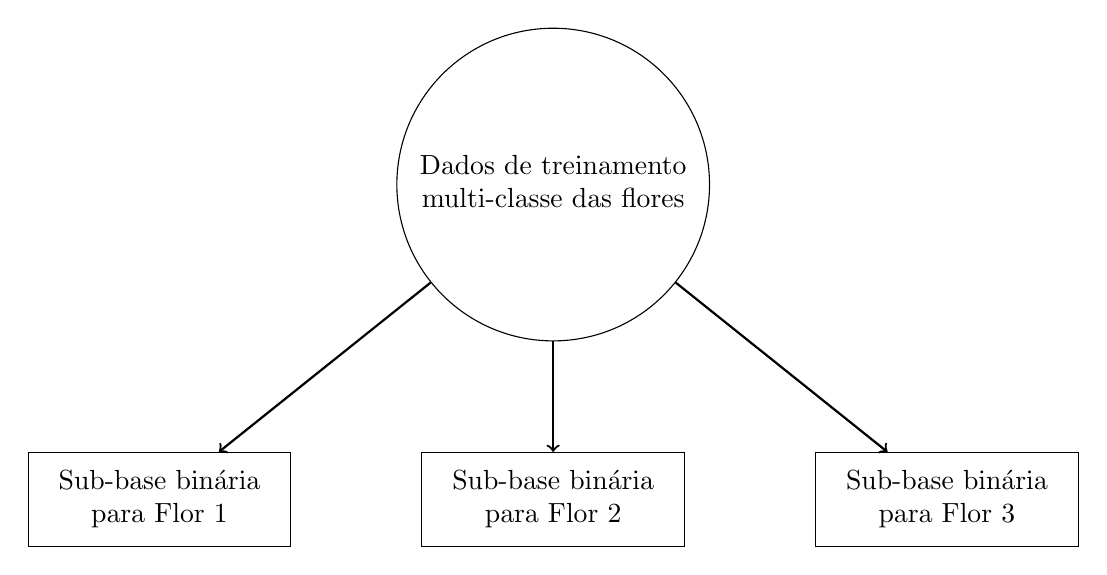
\begin{tikzpicture}
        % Original data node with tabular for line break
        \node[draw, circle, fill=white, inner sep=1pt] (original) at (0,0) {
            \begin{tabular}{c}
                Dados de treinamento \\
                multi-classe das flores
            \end{tabular}
        };

        % Split nodes
        \node[draw, rectangle, fill=white, inner sep=5pt] (split1) at (-5,-4) {
            \begin{tabular}{c}
                Sub-base binária \\
                para Flor 1
            \end{tabular}
        };
        \node[draw, rectangle, fill=white, inner sep=5pt] (split2) at (0,-4) {
            \begin{tabular}{c}
                Sub-base binária \\
                para Flor 2
            \end{tabular}
        };
        \node[draw, rectangle, fill=white, inner sep=5pt] (split3) at (5,-4) {
            \begin{tabular}{c}
                Sub-base binária \\
                para Flor 3
            \end{tabular}
        };

        % Arrows
        \draw[->, thick] (original) -- (split1) node[midway, above] {};
        \draw[->, thick] (original) -- (split2) node[midway, above] {};
        \draw[->, thick] (original) -- (split3) node[midway, above] {};
    \end{tikzpicture}
    \caption{Dividindo os dados de treinamento multi-classe das flores para sub-bases de treinamento binário para cada flor}
    \label{fig-flores}
\end{figure}

\section{Seleção das características}

Com a base de treinamento pronta e sub-divida, é feito a seleção das características para cada classificador de cada falha. Portanto, as características são ranqueadas pelo nível de manifestação obtida através dos dados quando uma falha ocorre. Neste estudo cientifico, foi utilizado cinco métodos de seleção e estes receberam os mesmos dados sem modificações.

\section{Treinamento dos classificadores}

Depois da retirada de características que não contribuem para identificação, os classificadores são treinados com os dados de sua respectiva falha. Nesse caso, o classificador torna-se especialista da classe positiva que corresponde a falha selecionada, conseguindo identificar essa falha dentre as demais. Nesse processo, foi criado diversos classificadores para a mesma falha, mas com a quantidade de características diferentes, seguindo o ranqueamento feito na seleção. Com isso, esse conjunto de classificadores terão diferentes taxas de acerto, mas apenas o melhor é selecionado.

\section{Seleção do melhor classificador}

Após o treinamento dos classificadores, é metrificado a acurácia com a base de testes. Nisso, são selecionados os melhores classificadores baseados em sua taxa de acerto para cada falha. Utilizando novamente como exemplo a base das flores, suponha que para a primeira flor, foi criado diversos classificadores binários especializados em identificar esse tipo de flor, mas com diferentes quantidades de características que foram utilizadas em seu treinamento. Entretanto, apenas um classificador foi escolhido para ser utilizado em identificar novas flores. Portanto, esse classificador é selecionado para compor o conjunto de classificadores que serão responsáveis em identificar as três flores.